\chapter{Global Project Organization}
\label{vl:tc-global}


\section{DUNE Management}
\label{sec:dune_management}

EB, Consortia, TB, ....

Relation to EFIG...

The high level organization of \dword{lbnf} and \dword{dune} is shown
in Fig~\ref{fig:DUNE_org_chart}. This shows the relationship of the
\dword{dune} management to that of \dword{lbnf} and the Joint Project
Office.
\begin{dunefigure}[Overall \dword{lbnf}/\dword{dune} organization]{fig:DUNE_org_chart}
  {Overall \dword{lbnf}/\dword{dune} organization.}
  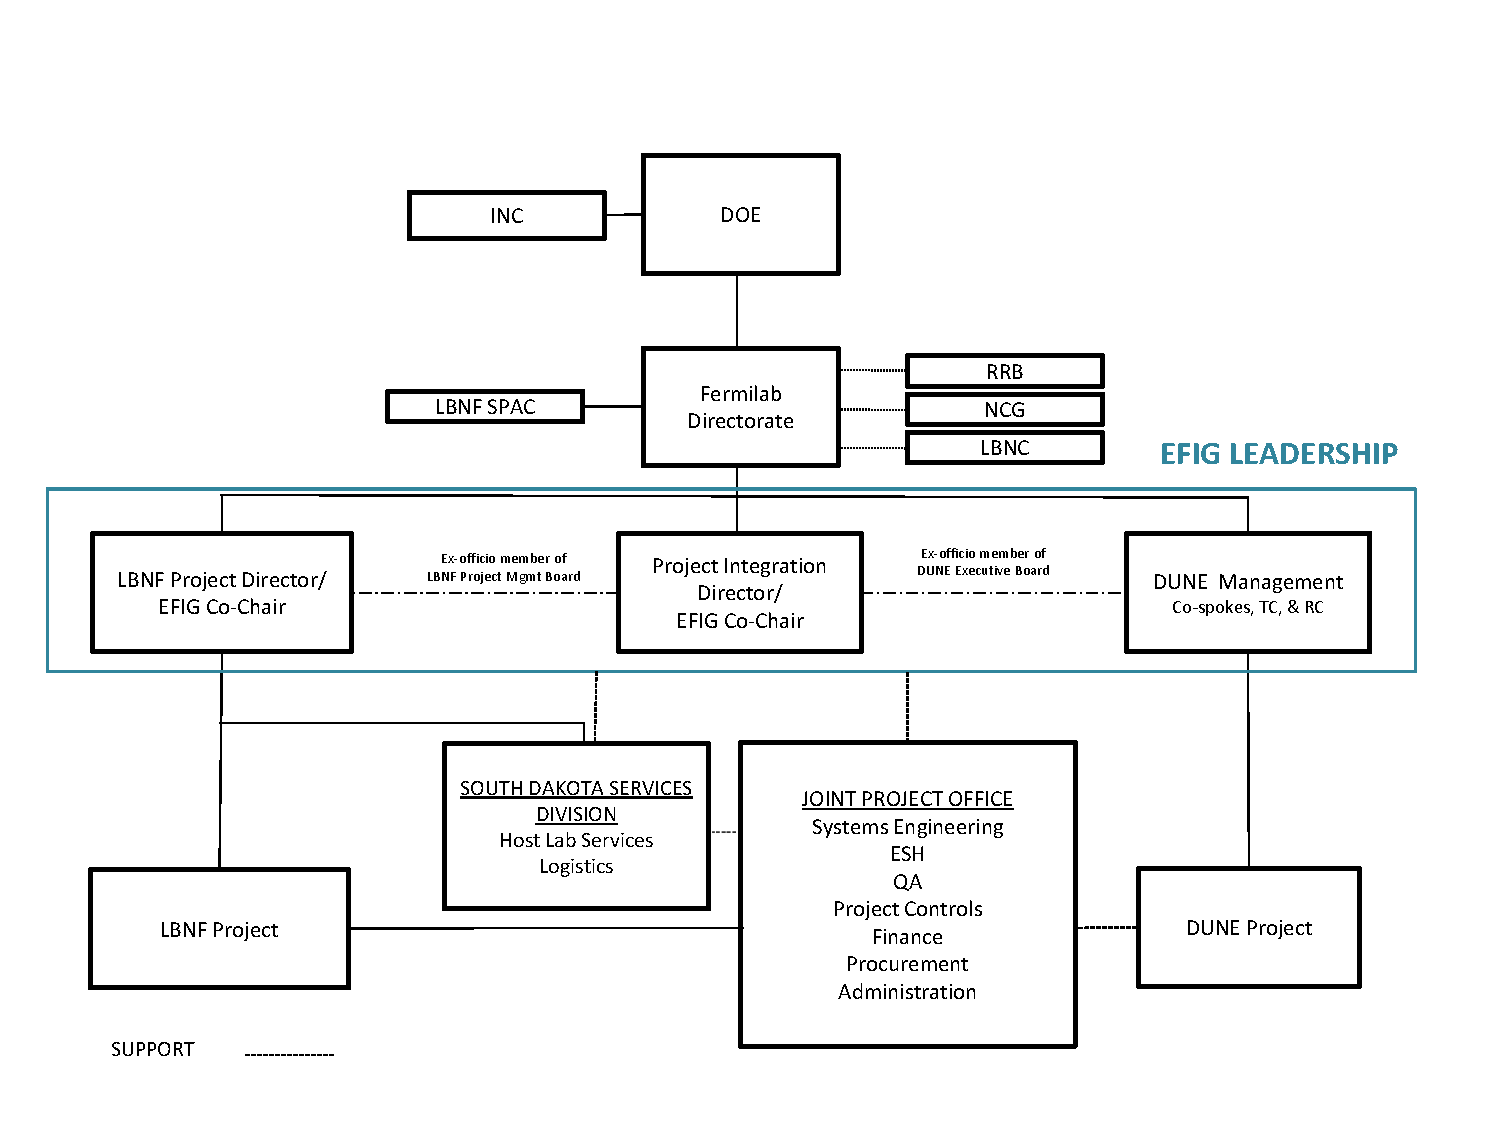
\includegraphics[width=0.99\textwidth]{DUNE_org_chart}
\end{dunefigure}

%\section{Consortia}
\section{DUNE Far Detector Consortia}
\label{sec:consortia}


Construction of the \dword{dune} far \dwords{detmodule} is carried out by
``consortia of collaboration institutions'' who assume responsibility
for detector subsystems.  Each consortium plans and
executes the construction, installation and commissioning of its 
subsystem.


A total of eleven \dword{fd} consortia have been formed to cover the
subsystems required for the two \dword{lartpc} designs, \dword{sp} and
\dword{dp}, currently under consideration.  Three consortia pursue
subsystems specific to the \dword{sp} design (\dword{apa}, \dword{ce},
and \dword{pds}) and another three consortia pursue designs for
\dword{dp} specific subsystems (\dword{crp}, TPC electronics and a
\dword{dp} \dword{pds}).  An additional five consortia are responsible
for subsystems common to both detector technologies; these are
\dword{hv}, \dword{daq}, \dword{cisc}, calibration and computing.



A consortium leader and a technical lead manage each consortium.  The
consortium leader chairs an institutional board composed of one
representative from each of the contributing institutions.
Significant consortium decisions, such as technology selections and
assignment of responsibilities among the institutions, are first
passed through this board, then passed as recommendations to the
\dword{dune} \dword{exb} for formal collaboration approval.


In many cases, multiple institutions within a consortium, potentially
supported by different funding agencies, share responsibility for a
particular subsystem deliverable.  \dword{dune} expects each
participating funding agency to manage its own internal project
responsibilities.  The consortium technical lead coordinates the
separate internal projects. This person also chairs a consortium
project management board, composed of the managers of each internal
project, that oversees the interconnections between the different
efforts.


%\section{(suggested) Executive Board}

The \dword{dune} \dword{exb} is the primary collaboration
decision-making body and as such includes representatives from all
major areas of activity within the collaboration.  All collaboration
decisions, especially those with potential impact on the \dword{dune}
scientific program or connected with the assignment of institutional
responsibilities, pass through the \dword{exb}.  \dword{exb} decisions
are expected to be achieved through consensus.  In cases where
consensus cannot be obtained, decision-making responsibility passes to
the co-spokespersons.  The consortium leader represents the consortium
on the \dword{exb}.

\section{Global Project Partners}
\label{sec:partners}

\fixme{with this section heading, I'd expect something about
  international funding agencies...this info could go up top in my
  suggested section}

The \dword{lbnf} project is responsible for providing conventional
facilities and supporting infrastructure (cryostats and cryogenic
systems) that house the \dword{dune} \dword{fd} modules. \dword{lbnf}
is a \dword{us} DOE project incorporating in-kind contributions from
international partners and is headed by the \dword{lbnf} project
director, who also serves as the \dword{fnal} deputy director for
\dword{lbnf}.  Conversely, \dword{dune} is an international project
directed by the \dword{dune} collaboration management team, with some
\dword{us} DOE contributions.

The \dword{efig} is responsible for high-level coordination between
the \dword{lbnf} and \dword{dune} projects.  The \dword{efig} is
co-chaired by the \dword{lbnf} project director and the integration
project director, who is appointed by and reports to the \dword{fnal}
director, and is responsible for the integration and installation of
the detector modules and for supporting the \dword{lbnf}
infrastructure in the underground areas at \dword{surf},
post-excavation.  The integration project director is connected to the
facilities and detector construction projects through their ex-officio
positions on the \dword{lbnf} project management board and
\dword{dune} \dword{exb}, respectively.

\dword{efig} leadership incorporates the four members of the
\dword{dune} collaboration management team (co-spokespersons,
\dword{tcoord} and \dword{rcoord}).  The \dword{efig} is responsible
for steering the global project and operates via consensus.  If
consensus cannot be achieved for a given issue, responsibility for
resolving the issue is passed to the \dword{fnal} director.

The \dword{efig} is supported by the \dword{jpo}, headed by the
integration project director.  \dword{jpo} functions include global
project configuration and integration, installation planning and
coordination, scheduling, safety assurance, technical review planning
and oversight, development of partner agreements, and financial
reporting.  The \dword{jpo} teams covering each of these areas are
formed from the members of the \dword{lbnf} project and \dword{dune}
\dword{tc} teams with responsibilities in these same areas.  For
example, the \dword{jpo} team responsible for building the fully
integrated model of the detector within its supporting infrastructure
and the surrounding facility includes members of the \dword{lbnf}
project and \dword{dune} \dword{tc} teams responsible for integrating
the individual elements.

%%%%%%%%%%%%%%%%%%%%%%%%%%%%%%%%
\section{Schedule}
\label{sec:fdsp-coord-schedule}

A series of tiered milestones have been developed for the \dword{dune}
project. The spokespersons and host laboratory director are
responsible for the tier 0 milestones. Three tier 0 milestones have
been defined and the dates set:
\begin{enumerate}
\item Start main cavern excavation \hspace{2.58in} 20xx
\item Start \dword{detmodule}~1 installation \hspace{2.1in} 20xx
\item Start operations of \dwords{detmodule} \#1--2 with beam \hspace{0.8in} 20xx
\end{enumerate}
These dates will be revisited this spring before the \dword{tdr} is reviewed. The
dword{tcoord} and \dword{lbnf} project manager hold the Tier 1
milestones; these milestones will be defined in advance of the
\dword{tdr} review. The consortia themselves hold the Tier 2
milestones.

Table~\ref{tab:DUNE_schedule} provides a high level version of the
\dword{dune} milestones from the \dword{ims}.
\begin{dunetable}
  [Overall \dword{dune} Project Tier-1 milestones.]
  {p{0.84\linewidth}p{0.14\linewidth}}
  {tab:DUNE_schedule}
  {Overall \dword{dune} Project Tier-1 milestones.}
  Milestone & Date   \\ \toprowrule
  RRB Approval of Technical Design Review                       &  \\ \colhline
  Beneficial Occupancy of Integration Test Facility             &  \\ \colhline
  Construction of steel frame for Cryostat \#1 complete         &  \\ \colhline
  Beneficial Occupancy of Central Utility Cavern Counting room  &  \\ \colhline
  Construction of steel frame for Cryostat \#2 complete         &  \\ \colhline
  \textbf{Beneficial occupancy of Cryostat \#1}                 & \textbf{} \\ \colhline
  Cryostat \#1 ready for TPC installation                       &  \\ \colhline
  \textbf{Beneficial occupancy of Cryostat \#2}                 & \textbf{} \\ \colhline
  Cryostat \#2 ready for TPC installation                       &  \\ \colhline
  Cryostat \#1 ready for filling                                &  \\ \colhline
  \textbf{Detector \#1 ready for operations}                    & \textbf{} \\ \colhline
  Cryostat \#2 ready for filling                                &  \\ \colhline
  \textbf{Detector \#2 ready for operations}                    & \textbf{} \\
\end{dunetable}
To monitor progress, \Dword{tc} will maintain the \dword{ims} that
links all consortium schedules and contains milestones for each
consortia.  The schedules will go under change control after each
consortium agrees to the milestone dates and the \dword{tdr} is
approved.  In addition to the overall \dword{ims} for construction and
installation, a schedule of key consortia activities has been
developed during 2018 and 2019.

To ensure that the \dword{dune} detector remains on schedule,
\dword{tc} will monitor schedule status from each consortium and organize
reviews of schedules and risks as appropriate.  As schedule problems
arise, \dword{tc} will work with affected consortium to resolve the
problems. If problems cannot be solved, the \dword{tc} will take the issue to the
\dword{tb} and \dword{exb}.

A monthly report with input from all consortia will be published by
\dword{tc}. This will include updates on consortium and \dword{tc}
technical progress against the \dword{ims}.

%%%%%%%%%%%%%%%%%%%%%%%%%%%%%%%%
\section{Requirements}
\label{sec:fdsp-coord-requirements}

%%%%%%%%%%%%%%%%%%%%%%%%%%%%%%%%
\section{Change Control}
\label{sec:fdsp-coord-change}

%%%%%%%%%%%%%%%%%%%%%%%%%%%%%%%%
\section{ProtoDUNE Lessons Learned}
\label{sec:fdsp-coord-lessonslearned}
